\begin{name}
	{ÔN TẬP KIỂM TRA CUỐI HỌC KÌ 1 - KNTT}
	{TOÁN 10}
	{LỚP TOÁN THẦY PHÁT}
	{\thoigian}
\end{name}

\caulc
\Opensolutionfile{ans}[ans/10-CK1-Chuyen-Hung-Vuong-Phan-1]
%%%============EX_1==============%%%
\begin{ex}%[0H4N2-2]%[Đề cuối kì 1 - Lớp 10 - năm học: 2024-2025 - Chuyên Hùng Vương - Phú Thọ]%[Tex hoá: Dương Công Tạo]
	Cho $\mathit{\Delta}ABC$ có $a=8$, $c=5$, $\widehat{B}=60^\circ $. Diện tích của tam giác $ABC$ bằng
	\choice
	{$20\sqrt{3}$}
	{$10$}
	{\True $10\sqrt{3}$}
	{$20$}
	\loigiai{
		Diện tích của tam giác $ABC$ là $S=\dfrac{1}{2}\cdot a\cdot c\cdot \sin B=\dfrac{1}{2}\cdot 8\cdot 5\cdot \sin 60^\circ=10\sqrt{3}$.
	}
\end{ex}
%%%============EX_2==============%%%
\begin{ex}%[0D1H2-1]%[Đề cuối kì 1 - Lớp 10 - năm học: 2024-2025 - Chuyên Hùng Vương - Phú Thọ]%[Tex hoá: Dương Công Tạo]
	 Cho tập hợp $A=\left\{x\in \mathbb{R}\mid(x-2)\left(x^2-1\right)=0\right\}$. Khẳng định nào dưới đây đúng? 
	\choice
	{$A=\{-1;1;-2\}$}
	{$A=\left\{-1;1\right\}$}
	{$A=\{2\}$}
	{\True $A=\{-1;1;2\}$}
	\loigiai{
		Xét tập hợp $A=\left\{x\in \mathbb{R}\mid(x-2)\left(x^2-1\right)=0\right\}$, ta có
		\begin{align*}
			(x-2)\left(x^2-1\right)=0\Leftrightarrow\hoac{&x-2=0\\&x^2-1=0}\Leftrightarrow\hoac{&x=2\\&x=\pm 1.}
		\end{align*}
	Mà $x\in \mathbb{R}$ nên $A=\{-1;1;2\}$.
	}
\end{ex}
%%%============EX_3==============%%%
\begin{ex}%[0H4H2-1]%[Đề cuối kì 1 - Lớp 10 - năm học: 2024-2025 - Chuyên Hùng Vương - Phú Thọ]%[Tex hoá: Dương Công Tạo]
	Cho tam giác $ABC$ có $\widehat{ABC}=45^\circ$, $\widehat{ACB}=60^\circ$ và $AB=3$. Tính $AC$.
	\choice
	{\True $AC=\sqrt{6}$}
	{$AC=3\sqrt{2}$}
	{$AC=6$}
	{$AC=2\sqrt{3}$}
	\loigiai{
		Áp dụng định lí sin, ta có \begin{eqnarray*}
			\dfrac{AB}{\sin C}=\dfrac{AC}{\sin B}&\Leftrightarrow& AC=\dfrac{AB}{\sin C}\cdot \sin B\\
			&\Leftrightarrow& AC=\dfrac{3}{\sin 60^\circ}\cdot \sin 45^\circ\\
			&\Leftrightarrow& AC=\sqrt{6}.
		\end{eqnarray*}
	}
\end{ex}
%%%============EX_4==============%%%
\begin{ex}%[0D6N4-1]%[Đề cuối kì 1 - Lớp 10 - năm học: 2024-2025 - Chuyên Hùng Vương - Phú Thọ]%[Tex hoá: Dương Công Tạo]
	Số đặc trưng nào sau đây đo độ phân tán của mẫu số liệu?
	\choice
	{Trung vị}
	{Mốt}
	{Số trung bình}
	{\True Độ lệch chuẩn}
	\loigiai{
		Số đặc trưng đo độ phân tán của mẫu số liệu là độ lệch chuẩn.
	}
\end{ex}
%%%============EX_5==============%%%
\begin{ex}%[0D2N1-1]%[Đề cuối kì 1 - Lớp 10 - năm học: 2024-2025 - Chuyên Hùng Vương - Phú Thọ]%[Tex hoá: Dương Công Tạo]
	Trong các bất phương trình dưới đây, bất phương trình nào là bất phương trình bậc nhất hai ẩn?
	\choice
	{$x-\dfrac{2}{y}\ge 3$}
	{\True $x-2y\ge 3$}
	{$x^2-2y\ge 3$}
	{$\sqrt{x}-2y\ge 3$}
	\loigiai{
		Bất phương trình $x-2y\ge 3$ là bất phương trình bậc nhất hai ẩn.
	}
\end{ex}
%%%============EX_6==============%%%
\begin{ex}%[0H4H1-2]%[Đề cuối kì 1 - Lớp 10 - năm học: 2024-2025 - Chuyên Hùng Vương - Phú Thọ]%[Tex hoá: Dương Công Tạo]
	Cho $\alpha$ là góc tù và $\sin\alpha=\dfrac{5}{13}$. Tính $\cos\alpha$.
	\choice
	{\True $\cos\alpha=-\dfrac{12}{13}$}
	{$\cos\alpha=-\dfrac{8}{13}$}
	{$\cos\alpha=\dfrac{12}{13}$}
	{$\cos\alpha=\dfrac{8}{13}$}
	\loigiai{
		Ta có
		\begin{itemize}
			\item $\alpha$ là góc tù nên $\cos\alpha<0$.
			\item $\cos\alpha=-\sqrt{1-\sin^2\alpha}=-\dfrac{12}{13}$.
		\end{itemize}
		
	}
\end{ex}
%%%============EX_7==============%%%
\begin{ex}%[0D6N3-2]%[Đề cuối kì 1 - Lớp 10 - năm học: 2024-2025 - Chuyên Hùng Vương - Phú Thọ]%[Tex hoá: Dương Công Tạo]
	Mẫu số liệu sau cho biết số ghế trống tại một rạp chiếu phim trong $9$ ngày
	\begin{center}
		$\begin{array}{|c|c|c|c|c|c|c|c|c|}
		\hline
		9 & 8 & 22 & 20 & 18 & 15 & 19 & 13 & 11 \\
		\hline
	\end{array}$
	\end{center}
	Số ghế trống trung bình trong $9$ ngày của rạp chiếu phim trên là
	\choice
	{$22$}
	{$18$}
	{\True $15$}
	{$135$}
	\loigiai{
		Số ghế trống trung bình trong $9$ ngày của rạp chiếu phim trên là
		\begin{align*}
			\overline{x}=\dfrac{1}{9}\left(8+9+11+13+15+18+19+20+22\right)=15.
		\end{align*}
	}
\end{ex}
%%%============EX_8==============%%%
\begin{ex}%[0D1N1-3]%[Đề cuối kì 1 - Lớp 10 - năm học: 2024-2025 - Chuyên Hùng Vương - Phú Thọ]%[Tex hoá: Dương Công Tạo]
	Mệnh đề phủ định của mệnh đề \lq\lq $\sqrt{2}$ là số vô tỉ\rq\rq\, là
	\choice
	{$\sqrt{2}$ là số thực}
	{$\sqrt{2}$ là số nguyên}
	{\True $\sqrt{2}$ không phải là số vô tỉ}
	{$\sqrt{2}$ không phải là số thực}
	\loigiai{
		\lq\lq$\sqrt{2}$ không phải là số vô tỉ\rq\rq\, là mệnh đề phủ định của mệnh đề \lq\lq $\sqrt{2}$ là số vô tỉ\rq\rq.
	}
\end{ex}
%%%============EX_9==============%%%
\begin{ex}%[0H5H2-2]%[Đề cuối kì 1 - Lớp 10 - năm học: 2024-2025 - Chuyên Hùng Vương - Phú Thọ]%[Tex hoá: Dương Công Tạo]
	Cho tam giác $ABC$, khẳng định nào sau đây đúng?
	\choice
	{$\overrightarrow{AB}-\overrightarrow{AC}=\overrightarrow{BC}$}
	{$\overrightarrow{AB}-\overrightarrow{CA}=\overrightarrow{BC}$}
	{\True $\overrightarrow{BC}+\overrightarrow{AB}=\overrightarrow{AC}$}
	{$\overrightarrow{AB}+\overrightarrow{AC}=\overrightarrow{CB}$}
	\loigiai{
		Ta có $\overrightarrow{BC}+\overrightarrow{AB}=\overrightarrow{AB}+\overrightarrow{BC}=\overrightarrow{AC}$.
	}
\end{ex}
%%%============EX_10==============%%%
\begin{ex}%[0D2H2-3]%[Đề cuối kì 1 - Lớp 10 - năm học: 2024-2025 - Chuyên Hùng Vương - Phú Thọ]%[Tex hoá: Dương Công Tạo]
	Một cửa hàng dự định kinh doanh hai loại máy điều hòa: điều hòa một chiều và điều hòa hai chiều. Khảo sát thị trường cửa hàng thấy nhu cầu của thị trường sẽ không vượt quá $100$ máy cả hai loại. Gọi $x$, $y$ lần lượt là số máy điều hòa một chiều và điều hòa hai chiều mà cửa hàng nhập vào. Khi đó, $(x;y)$ là nghiệm của hệ bất phương trình nào dưới đây?
	\choice
	{\True $\heva{&{x\ge 0} \\
			&{y\ge 0} \\
			&{x+y\le 100}
			&}$}
	{$\heva{&{x\ge 0} \\
			&{y\ge 0} \\
			&{x+y < 100}
			&}$}
	{$\heva{&{x\ge 0} \\
			&{y\ge 0} \\
			&{x+y\ge 100}
			&}$}
	{$\heva{&{x\ge 0} \\
			&{y\ge 0} \\
			&{x+y > 100}
			&}$}
	\loigiai{
		Theo giả thiết, ta có $(x;y)$ là nghiệm của hệ bất phương trình $\heva{&{x\ge 0} \\
			&{y\ge 0} \\
			&{x+y\le 100.}
			&}$
	}
\end{ex}
%%%============EX_11==============%%%
\begin{ex}%[0D2H2-2]%[Đề cuối kì 1 - Lớp 10 - năm học: 2024-2025 - Chuyên Hùng Vương - Phú Thọ]%[Tex hoá: Dương Công Tạo]
	Cho hệ bất phương trình $\heva{&x-y <-3 \\&2y\ge-4.}$ \\
		Điểm nào sau đây thuộc miền nghiệm của hệ bất phương trình đã cho?
		\choice
		{$(3;-1)$}
		{$(-2;1)$}
		{\True $(-3;1)$}
		{$(0;0)$}
	\loigiai{
		Vì $\heva{&-3-1 <-3\text{ (đúng)} \\&2\cdot 1\ge-4\text{ (đúng)}.}$\\
		nên điểm $(-3;1)$ thuộc miền nghiệm của hệ bất phương trình đã cho.
	} 
\end{ex}
%%%============EX_12==============%%%
\begin{ex}%[0H5N1-3]%[Đề cuối kì 1 - Lớp 10 - năm học: 2024-2025 - Chuyên Hùng Vương - Phú Thọ]%[Tex hoá: Dương Công Tạo]
	\immini[thm]{Cho hình vuông $ABCD$ có tâm $O$ (hình vẽ). 
		Vectơ $\overrightarrow{AO}$ bằng vectơ
		\choice
		{$\overrightarrow{OD}$}
		{$\overrightarrow{CO}$}
		{$\overrightarrow{OB}$}
		{\True $\overrightarrow{OC}$}}
	{\begin{tikzpicture}[scale=.7]
			\def\a{4}
			\path 	(0:0) coordinate (A)
			(0:\a) coordinate (B)
			(-90:\a) coordinate (D)
			($(D)-(A)+(B)$) coordinate (C)
			(intersection of A--C and B--D) coordinate (O);
			\draw	(A)--(B)--(C)--(D)--cycle (A)--(C)	(B)--(D);
			\foreach \x/\g in {A/135,B/45,C/-45,D/-135,O/90}
			\fill[black] 	(\x) circle (1pt)
			($(\g:4mm)+(\x)$) node {$\x$};	
		\end{tikzpicture}
	}
	\loigiai{
		Quan sát hình vẽ, ta thấy $\overrightarrow{OC}=\overrightarrow{AO}$.
	}
\end{ex}
\Closesolutionfile{ans}
% \indapan{7}{ans/10-CK1-Chuyen-Hung-Vuong-Phan-1}

\cauds
\Opensolutionfile{ans}[ans/10-CK1-Chuyen-Hung-Vuong-Phan-2]
\begin{ex}%[0D6H4-4]%[Đề Cuối kì 1 - Lớp 10 - năm học 2024 - 2025 - Chuyên Hùng Vương - Phú Thọ]%[Tex hóa: Lê Thị Thúy Hằng]
Kết quả kiểm tra cuối kì I môn Toán (thang điểm 10) của hai lớp $10$A và $10$B được thống kê như sau:\\
%\begin{center}
	\begin{minipage}{7cm}
		{\begin{center}
			\begin{tabular}{|c|c|c|c|c|}
				\hline
				$2$ & $7$ & $6$ & $3$ & $9$ \\
				\hline
				$8$ & $6$ & $7$ & $9$ & $2$ \\
				\hline
				$5$ & $7$ & $5$ & $9$ & $8$ \\
				\hline
				$8$ & $7$ & $4$ & $3$ & $5$ \\
				\hline
				$5$ & $4$ & $5$ & $7$ & $7$ \\
				\hline
			\end{tabular}
			\\ Lớp 10A
		\end{center}			
		}
	\end{minipage}
	\begin{minipage}{7cm}
		{\begin{center}
			\begin{tabular}{|c|c|c|c|c|}
				\hline
				$6$ & $7$ & $6$ & $4$ & $7$\\
				\hline
				$9$ & $3$ & $8$ & $7$ & $5$\\
				\hline
				$5$ & $6$ & $8$ & $7$ & $4$\\
				\hline
				$5$ & $3$ & $10$ & $7$ & $9$\\
				\hline
				$6$ & $7$ & $6$ & $7$ & $5$\\
				\hline
			\end{tabular}
			\\ Lớp 10B
		\end{center}
		}
	\end{minipage}
%\end{center}
	\choiceTF
		{\True Trung vị của mẫu số liệu ở lớp $10$B là $6$}
		{\True Điểm trung bình môn Toán của lớp 10A là $5{,}92$}
		{Điểm kiểm tra cuối kì I môn Toán lớp $10$A đồng đều hơn lớp $10$B}
		{Mốt của mẫu số liệu ở lớp $10$A nhỏ hơn mốt của mẫu số liệu ở lớp $10$B}
		\loigiai{
		\begin{itemchoice}
			\itemch Đúng.\\
			%Sắp xếp điểm của lớp $10$A theo thứ tự không giảm:
			%$$2; 2; 3; 3; 4; 4; 5; 5; 5; 5; 5; 6; 6; 7; 7; 7; 7; 7; 7; 8; 8; 8; 9; 9; 9.$$
			Sắp xếp điểm của lớp $10$B theo thứ tự không giảm
			$$3; 3; 4; 4; 5; 5; 5; 5; 6; 6; 6; 6; 6; 7; 7; 7; 7; 7; 7; 7; 8; 8; 9; 9; 10.$$
			Trung vị của mẫu số liệu ở lớp $10$B là $x_{13}=6$.
			\itemch Đúng.
			Ta có\\
			$\overline{x}_{10A} = \dfrac{2 \cdot 2 + 3 \cdot 2 + 4 \cdot 2 + 5 \cdot 5 + 6 \cdot 2 + 7 \cdot 6 + 8 \cdot 3 + 9 \cdot 3}{25} = 5{,}92$.\\
			$\overline{x}_{10B} = \dfrac{3 \cdot 2 + 4 \cdot 2 + 5 \cdot 4 + 6 \cdot 5 + 7 \cdot 7 + 8 \cdot 2 + 9 \cdot 2 + 10 \cdot 1}{25} = 6{,}28$.\\
			\itemch Sai.\\
			Ta lập bảng tần số\\
			{\tabcolsep = 3mm
				\begin{tabular}{|c|c|c|c|c|c|c|c|c|c|}
					\hline
					Điểm & $2$ & $3$ & $4$ & $5$ & $6$ & $7$ & $8$ & $9$ & $10$ \\
					\hline Số học sinh lớp $10$A & $2$ & $2$ & $2$ & $5$ & $2$ & $6$ & $3$ & $3$ & $0$\\
					\hline Số học sinh lớp $10$B & $0$ & $2$ & $2$ & $4$ & $5$ & $7$ & $2$ & $2$ & $1$  \\
					\hline
				\end{tabular}
			}
			
			Ta có
			\begin{eqnarray*}
				S^2_{10A} & = & \dfrac{1}{25} [ (2-5{,}92)^2 + (3-5{,}92)^2 +(4-5{,}92)^2 +(5-5{,}92)^2  \\
				& & +(6-5{,}92)^2 +(7-5{,}92)^2 +(8-5{,}92)^2 +(9-5{,}92)^2 ] \\
				& = & 4{,}3136;\\
				S^2_{10B} & = & \dfrac{1}{25} [ (3-6{,}28)^2 + (4-6{,}28)^2 + (5-6{,}28)^2 +(6-6{,}28)^2 \\
				& & + (7-6{,}28)^2 + (8-6{,}28)^2 +(9-6{,}28)^2 +(10-6{,}28)^2] \\
				& = & 3{,}0816.
			\end{eqnarray*}
			Vì $S^2_{10A} > S^2_{10B}$ nên điểm kiểm tra cuối kì I môn Toán lớp $10$B đồng đều hơn lớp $10$A.
			\itemch Sai.\\
			Mốt của mẫu số liệu của lớp $10$A là $M_0=7$.\\
			Mốt của mẫu số liệu của lớp $10$B là $M_0=7$.\\
			Do đó, mốt của mẫu số liệu của lớp $10$A và mốt của mẫu số liệu của lớp $10$B bằng nhau.
		\end{itemchoice}
		}
\end{ex}
% \begin{ex}%[0D2V2-2]%[Đề Cuối kì 1 - Lớp 10 - năm học 2024 - 2025 - Chuyên Hùng Vương - Phú Thọ]%[Tex hóa: Lê Thị Thúy Hằng]
% 	Cho $(x;y)$ là nghiệm của hệ bất phương trình $\heva{
% 		&-2x+y \le 2\\
% 		&x\le 5\\
% 		&y\le 4\\
% 		&x+y\ge-1.
% 	}$
% 	\choiceTF
% 	{\True Biểu thức $F(x;y)=-x-y$ đạt giá trị lớn nhất bằng $1$}
% 	{Biểu thức $F(x;y)=-x-y$ đạt giá trị nhỏ nhất khi $x=5$; $y=-6$}
% 	{Miền nghiệm của hệ là miền tam giác (tính cả cạnh)}
% 	{\True Cặp số $(x;y)=(0;0)$ là nghiệm của hệ}
% 	\loigiai{
% 	Đặt $d_1 \colon -2x+y-2=0$, $d_2 \colon x+y+1=0$.
% 	Ta có miền nghiệm của hệ bất phương trình được biểu diễn trong hình dưới
% 	\begin{center}
% 		\begin{tikzpicture}[line join=round, line cap=round,>=stealth,thick]
% 			\tikzset{every node/.style={scale=0.6}}
% 			\begin{scope}
% 				\clip (-2,-7) rectangle (6,5);
% 				\fill[pattern=dots] (-5,-8)--(-5,16)--(7,16)--cycle;
% 				\fill[pattern=dots] (5,-7)--(6,-7)--(6,7)--(5,7)--cycle;
% 				\fill[pattern=dots] (-2,4)--(-2,7)--(6,7)--(6,4)--cycle;
% 				\fill[pattern=dots] (-9,8)--(-9,-8)--(7,-8)--cycle;
% 				\draw (1.5,5)--(-2,-2) node [pos=0.9, above, sloped] {$d_1$};
% 				\draw (5,-7)--(5,5) node [pos=0.2, above, sloped] {$x-5=0$};
% 				\draw (-2,4)--(6,4) node [pos=0.1, above, sloped] {$y-4=0$};
% 				\draw (-2,1)--(6,-7) node [pos=0.9, above, sloped] {$d_2$};
% 			\end{scope}
% 			\draw[->] (-2,0)--(6,0) node[below]{$x$};
% 			\draw[->] (0,-7)--(0,5) node[left]{$y$};
% 			\draw (0,0) node[below left]{$O$};
% 			\foreach \x in {-1,1,5}
% 			\draw[thin] (\x,1pt)--(\x,-1pt) node [below left] {$\x$};
% 			\foreach \y in {-6,2,4}
% 			\draw[thin] (1pt,\y)--(-1pt,\y) node [above left] {$\y$};
% 			\draw[dashed,thin] (0,4)-|(1,0);
% 			\draw[dashed,thin] (0,-6)-|(5,0);
% 		\end{tikzpicture}
% 	\end{center}
% 	Miền nghiệm của hệ bất phương trình trên là miền tứ giác với các đỉnh có tọa độ $(1;0)$, $(1;4)$, $(5;4)$, $(5;-6)$.\\
% 	$F(1;0)=-1$, $F(1;4)=-1-4=-5$, $F(5;4)=-5-4=-9$, $F(5;-6)=-5+6=1$.
% 	\begin{itemchoice}
% 		\itemch Đúng.\\
% 		Biểu thức $F(x;y)=-x-y$ đạt giá trị lớn nhất bằng $1$ tại $(x;y)=(5;-6)$.
% 		\itemch Sai.\\
% 		Biểu thức $F(x;y)=-x-y$ đạt giá trị nhỏ nhất bằng $-9$ tại $(x;y)=(5;4)$.
% 		\itemch Sai.\\
% 		Theo hình vẽ, miền nghiệm của hệ bất phương trình là miền tứ giác (tính cả cạnh).
% 		\itemch Sai.\\
% 		Thay $(x;y)=(0;0)$ vào bất phương trình $x+y \ge -1$ ta có $0+0 \ge -1$ là mệnh đề sai nên cặp số $(x;y)=(0;0)$ không là nghiệm của hệ bất phương trình.
% 	\end{itemchoice}
% 	}
% \end{ex}
\begin{ex}%[0H4V3-1]%[Đề Cuối kì 1 - Lớp 10 - năm học 2024 - 2025 - Chuyên Hùng Vương - Phú Thọ]%[Tex hóa: Lê Thị Thúy Hằng]
Cho $\triangle ABC$ có $BC=8$, $AB=5$, $\widehat{ABC} = 60^\circ$. Gọi $D$ là chân đường phân giác trong góc kẻ từ đỉnh $A$ và $G$ là trọng tâm của tam giác $ABC$.
	\choiceTF
	{\True $\overrightarrow{DB}$ và $\overrightarrow{DC}$ ngược hướng}
	{\True $7\overrightarrow{DB} + 5 \overrightarrow{DC}= \overrightarrow{0}$}
	{$\overrightarrow{AD} = \dfrac{5}{12} \overrightarrow{AB} + \dfrac{7}{12} \overrightarrow{AC}$}
	{$\overrightarrow{BG} \cdot \overrightarrow{AD}=12$}
	\loigiai{
	\begin{center}
		\begin{tikzpicture}[scale=0.5,font=\tiny]
			\def\a{8}
			\def\c{5}
			\path 
			(0:0) coordinate (B)
			(60:\a) coordinate (A)
			(0:\c) coordinate (C)
			($(B)!5/12!(C)$) coordinate (D)
			($(B)!1/2!(C)$) coordinate (M)
			($(A)!2/3!(M)$) coordinate (G)
			;
			\draw (A)--(B)--(C)--cycle (M)--(A)--(D);
			\foreach \x/\g in {A/90,B/180,C/0,D/-120,M/-90,G/0} 
				\draw[fill=black] (\x) circle (0.05) +(\g:0.4) node{$\x$}
			;
		\end{tikzpicture}
	\end{center}
	\begin{itemchoice}
		\itemch Đúng.\\
		Sử dụng định lý cosin ta có
		\begin{eqnarray*}
			AC^2 & = & AB^2 + BC^2 - 2 \cdot AB \cdot BC \cdot \cos 60^\circ \\
			& = & 5^2 + 8^2 - 2 \cdot 5 \cdot 8 \cdot \frac{1}{2} \\
			& = & 25 + 64 - 40 = 49
		\end{eqnarray*}
		$\Rightarrow AC = 7$.\\
		Ta có $\dfrac{BD}{DC} = \dfrac{AB}{AC} = \dfrac{5}{7}$ và ba điểm $B$, $D$, $C$ thẳng hàng theo thứ tự đó nên 
		$\overrightarrow{DB} = - \dfrac{5}{7} \cdot \overrightarrow{DC}$. Do đó, $\overrightarrow{DB}$ và $\overrightarrow{DC}$ ngược hướng.
		\itemch Đúng.\\
		Từ $\overrightarrow{DB} = - \dfrac{5}{7} \cdot \overrightarrow{DC}$ suy ra $7\overrightarrow{DB} + 5 \overrightarrow{DC}= \overrightarrow{0}$.
		\itemch Sai.\\
		Ta có  $7\overrightarrow{DB} + 5 \overrightarrow{DC}= \overrightarrow{0} \Rightarrow \overrightarrow{BD} = \dfrac{5}{12} \overrightarrow{BC}$.\\
		\begin{eqnarray*}
			\overrightarrow{AD} & = & \overrightarrow{AB} + \overrightarrow{BD}\\
			& = & \overrightarrow{AB} + \dfrac{5}{12} \overrightarrow{BC}\\
			& = & \overrightarrow{AB} + \dfrac{5}{12} \left( \overrightarrow{AC} - \overrightarrow{AB} \right)\\
			& = & \dfrac{7}{12} \overrightarrow{AB} + \dfrac{5}{12} \overrightarrow{AC}.
		\end{eqnarray*}
		\itemch Sai.\\
		Ta có $\overrightarrow{BG} = \dfrac{1}{3} \left( \overrightarrow{BA} + \overrightarrow{BC} \right)$.\\
		$\overrightarrow{AD} = \overrightarrow{BD} - \overrightarrow{BA} = -\overrightarrow{BA} + \dfrac{5}{12} \overrightarrow{BC}$.\\
		\begin{eqnarray*}
			\overrightarrow{BG} \cdot \overrightarrow{AD} & = & \dfrac{1}{3} \left( \overrightarrow{BA} + \overrightarrow{BC} \right) \cdot \left( -\overrightarrow{BA} + \dfrac{5}{12} \overrightarrow{BC} \right)\\
			& = & \dfrac{1}{3} \left( -BA^2 + \dfrac{5}{12} BC^2 - \dfrac{7}{12} \overrightarrow{BC} \cdot \overrightarrow{BA} \right)\\
			& = & \dfrac{1}{3} \left( -25 + \dfrac{5}{12} \cdot 64 - \dfrac{7}{12} \cdot 8 \cdot 5 \cdot \dfrac{1}{2} \right)\\
			& = &  -\dfrac{10}{3}.
		\end{eqnarray*}
	\end{itemchoice}
	}
\end{ex}

% \begin{ex}%[0H4V3-1]%[Đề Cuối kì 1 - Lớp 10 - năm học 2024 - 2025 - Chuyên Hùng Vương - Phú Thọ]%[Tex hóa: Lê Thị Thúy Hằng]
% Cho tam giác $ABC$ có $BC=8$, $AB=5$, $\widehat{ABC} = 60^\circ$. Khi đó
% 	\choiceTF
% 	{\True Độ dài cạnh $AC=7$}
% 	{Điểm $N$ thoả mãn $\overrightarrow{NB} + 3 \overrightarrow{NC} =\overrightarrow{0}$. Độ dài $AN$ bằng $\sqrt{19}$}
% 	{\True Tam giác $ABC$ là tam giác nhọn}
% 	{\True Bán kính đường tròn nội tiếp tam giác $ABC$ bằng $\sqrt{3}$}
% 	\loigiai{
% 	\begin{center}
% 		\begin{tikzpicture}[scale=0.5,font=\tiny]
% 			\def\a{8}
% 			\def\c{5}
% 			\path 
% 			(0:0) coordinate (B)
% 			(60:\a) coordinate (A)
% 			(0:\c) coordinate (C)
% 			($(B)!3/4!(C)$) coordinate (N)
% 			%($(B)!1/2!(C)$) coordinate (M)
% 			%($(A)!2/3!(M)$) coordinate (G)
% 			;
% 			\draw (A)--(B)--(C)--cycle (A)--(N);
% 			\foreach \x/\g in {A/90,B/180,C/0,N/-90} 
% 			\draw[fill=black] (\x) circle (0.05) +(\g:0.4) node{$\x$}
% 			;
% 		\end{tikzpicture}
% 	\end{center}
% 		\begin{itemchoice}
% 			\itemch Đúng.\\
% 			Sử dụng định lý cosin ta có
% 			\begin{eqnarray*}
% 				AC^2 & = & AB^2 + BC^2 - 2 \cdot AB \cdot BC \cdot \cos 60^\circ \\
% 				& = & 5^2 + 8^2 - 2 \cdot 5 \cdot 8 \cdot \frac{1}{2} \\
% 				& = & 25 + 64 - 40 = 49
% 			\end{eqnarray*}
% 			$\Rightarrow AC = 7$.
% 			\itemch Sai.\\
% 			Vì $\overrightarrow{NB} + 3 \overrightarrow{NC} =\overrightarrow{0}$ nên $N$ nằm giữa $B$, $C$ và $BN= \dfrac{3}{4} BC$.\\
% 			Do đó, $BN = \dfrac{3}{4} \cdot 8 = 6$.\\
% 			Sử dụng định lý cosin ta có
% 			\begin{eqnarray*}
% 				AN^2 & = & BA^2 + BN^2 - 2 \cdot BA \cdot BN \cdot \cos 60^\circ \\
% 				& = & 5^2 + 6^2 - 2 \cdot 5 \cdot 6 \cdot \frac{1}{2} \\
% 				& = & 25 + 36 - 30 = 31
% 			\end{eqnarray*}
% 			$\Rightarrow AN = \sqrt{31}$.
% 			\itemch Đúng.\\
% 			Tam giác $ABC$ có $AB<AC<BC$ nên ta chỉ cần tính $\cos A$.\\
% 			Ta có 
% 			\begin{eqnarray*}
% 				\cos A & = & \dfrac{AB^2 + AC^2 - BC^2}{2 \cdot AB \cdot AC}\\
% 				& = & \dfrac{5^2 + 7^2 - 8^2}{2 \cdot 5 \cdot 7}\\
% 				& = & \dfrac{1}{7}
% 			\end{eqnarray*}
% 			$\Rightarrow \widehat{A} \approx 82^\circ < 90^\circ$.\\
% 			Do đó, tam giác $ABC$ là tam giác nhọn.
% 			\itemch Đúng.\\
% 			Diện tích tam giác $ABC$ bằng 
% 			$$S= \dfrac{1}{2} \cdot BA \cdot BC \cdot \sin \widehat{ABC} = \dfrac{1}{2} \cdot 5 \cdot 8 \cdot \dfrac{\sqrt{3}}{2} = 10 \sqrt{3}.$$
% 			Có $p= \dfrac{AB+AC+BC}{2} = \dfrac{5+8+7}{2} = 10$.\\
% 			Do đó, bán kính đường tròn nội tiếp tam giác $ABC$ bằng
% 			$$r= \dfrac{S}{p} = \dfrac{10 \sqrt{3}}{10}= \sqrt{3}.$$
% 		\end{itemchoice}
% 	}
% \end{ex}
\Closesolutionfile{ans}
% \indapan{3}{ans/10-CK1-Chuyen-Hung-Vuong-Phan-2}

\caukq
\Opensolutionfile{ans}[ans/10-CK1-Chuyen-Hung-Vuong-Phan-3]
\begin{ex}%[0D1H2-2]
Cho hai tập hợp $A=\left\{x\in\mathbb{R}\mid x^2-3x+2=0\right\}$, $B=\{n\in\mathbb{N}\mid n\le 5\}$. Tìm số tập con của tập $A\cap B$.
\shortans{$4$}
\loigiai{
Ta có $A=\{1;2\}$ và $B=\{0;1;2;3;4;5\}$.\\
Vậy $A\cap B=\{1;2\}$.\\
Vậy số tập con của $A\cap B$ là $2^2=4$. 
}
\end{ex}

\begin{ex}%[0D2V2-3]
Trong một tuần, bạn Mạnh có thể thu xếp được tối đa $12$ giờ để tập thể dục, bạn Mạnh có thể chơi cầu lông hoặc tập Gym. Cho biết, mỗi giờ chơi cầu lông sẽ tiêu hao được $300$ calo và mất $30$ (nghìn đồng) chi phí, mỗi giờ tập Gym sẽ tiêu hao được $750$ calo và mất $50$ (nghìn đồng) chi phí, tổng số calo bạn Mạnh tiêu hao trong một tuần không ít hơn $6000$ calo. Tính số tiền chi phí ít nhất (đơn vị: nghìn đồng) mà bạn Mạnh phải bỏ ra trong một tuần.
\shortans{$400$}
\loigiai{
Gọi $x$ (giờ) là số giờ bạn Mạnh chơi cầu lông, y (giờ) là số giờ bạn Mạnh tập Gym trong một tuần.\\
Hiển nhiên ta có $x\ge 0$ và $y\ge 0$.\\
Tổng số giờ bạn Mạnh tập thể dục trong một tuần là $x+y$ (giờ)\\
Do một tuần bạn Mạnh thu xếp được tối đa $12$ giờ để tập thể dục nên ta có bất phương trình sau $x+y\le 12$.\\
Do mỗi giờ chơi cầu lông tiêu hao $300$ calo nên với $x$ giờ chơi cầu lông sẽ tiêu hao $300x$ calo.\\
Mỗi giờ tập tạ tiêu hao $750$ calo nên với $y$ giờ tập Gym sẽ tiêu hao $750y$ calo.\\
Tổng số calo tiêu hao là $350x+700y$ (calo).\\
Mặt khác, Mạnh tổng số calo bạn Mạnh tiêu hao trong một tuần không ít hơn $6000$ calo. Vì vậy, ta có bất phương trình: $300x+750y\geq 6000$, tức là $x+2{,}5y\geq 20$.\\
Vậy ta có hệ bất phương trình là 
$\heva{&x \ge 0\\
	&y \ge 0\\
	&x+y \le 12\\
	&x+2{,}5 y \ge 20.
}$\\
Biểu diễn miền nghiệm của hệ trên mặt phẳng tọa độ $O x y$ ta được hình ảnh sau
\begin{center}
\begin{tikzpicture}[line join=round, line cap=round,>=stealth,thick,scale=0.5]
	\tikzset{every node/.style={scale=0.9}}
	\begin{scope}
		\clip (-0.5,-0.5) rectangle (14,14);
		\fill[pattern=north east lines]  (0,-0.5)--(-0.5,-0.5)--(-0.5,14)--(0,14)--cycle;
		\fill[pattern=north east lines]  (-0.5,0)--(-0.5,-0.5)--(14,-0.5)--(14,0)--cycle;
		\fill[pattern=north east lines] (-2.5,14.5)--(15,14.5)--(15,-3)--cycle;
		\fill[pattern=north east lines]  (-15.5,14.2)--(-15.5,-0.8)--(22,-0.8)--cycle;
		\draw (-2,14)--(12.5,-0.5) ;
		\draw (-15,14)--(21.25,-0.5) ;
	\end{scope}
	\draw[->] (-0.5,0)--(14,0) node[below]{$x$};
	\draw[->] (0,-0.5)--(0,14) node[left]{$y$};
	\draw (0,0) node[below left]{$O$};
	\foreach \x in {12}
	\draw[thin] (\x,1pt)--(\x,-1pt) node [below] {$\x$};
	\foreach \y in {12,8}
	\draw[thin] (1pt,\y)--(-1pt,\y) node [left] {$\y$};
	\coordinate (A) at (0,8);
	\coordinate (B) at (0,12);
	\coordinate (C) at (6.6666666667,5.33333333);
	%Gán nhãn.
	\foreach \x/\y in {A/40,B/30, C/90}{\fill (\x) circle (1pt) ($(\x)+(\y:0.5cm)$) node{$\x$};}
\end{tikzpicture}
\end{center}
Vậy, miền không gạch (miền tam giác $ABC$, bao gồm cả các cạnh) là phần giao miền nghiệm của các bất phương trình trong hệ và cũng là phần biểu diễn miền nghiệm của hệ bất phương trình trên.\\
Tọa độ các đỉnh của tứ giác đó là $O (0;0)$, $A(0;10);B (4;8);C(12;0)$.\\
Gọi $F$ là chi phí tập luyện.\\
Mỗi giờ chơi cầu lông sẽ tiêu hao được $300$ calo và mất $30$ (nghìn đồng) chi phí, mỗi giờ tập Gym sẽ tiêu hao được $750$ calo và mất $50$ (nghìn đồng) chi phí nên $F=30x+50y$.\\
Tính các giá trị của $F$ tại các đỉnh của tam giác ta có\\
Tại $A(0;8)$ thì $ F=30\cdot 0+50\cdot 8=400$.\\
Tại $B(0;12)$ thì $ F=30\cdot 0+50\cdot 12=600$.\\
Tại $C\left(\dfrac{20}{3};\dfrac{16}{3}\right)$ thì $ F=30\cdot \dfrac{20}{3}+50\cdot \dfrac{16}{3}=\dfrac{1400}{3}$.\\
$F$ đạt giá trị nhỏ nhất bằng $400$ tại $A(0;8)$.\\
Vậy Mạnh muốn chi phí tập luyện là ít nhất khi Mạnh không chơi cầu lông và Mạnh chỉ tập Gym $12$ giờ một tuần.
}
\end{ex}

% \begin{ex}%[0D1V3-5]
% 	Lớp $10$A có $35$ học sinh. Trong đợt đăng kí câu lạc bộ thể dục đầu năm, mỗi học sinh đăng kí từ một đến ba câu lạc bộ gồm: bóng đá, cầu lông, đá cầu. Thống kê theo từng câu lạc bộ có: $20$ học sinh đăng kí câu lạc bộ bóng đá; $15$ học sinh đăng kí câu lạc bộ cầu lông; $9$ học sinh đăng kí câu lạc bộ đá cầu. Thống kê theo nhóm hai câu lạc bộ có: $4$ học sinh đăng kí câu lạc bộ bóng đá và cầu lông; $4$ học sinh đăng kí câu lạc bộ cầu lông và đá cầu; $3$ học sinh đăng kí câu lạc bộ đá cầu và bóng đá. Hỏi có bao nhiêu học sinh đăng kí cả ba câu lạc bộ?
% \shortans{$2$}
% \loigiai{
% Gọi
% $A$ là tập hợp học sinh đăng ký bóng đá.\\
% $B$ tập hợp học sinh đăng ký cầu lông.\\
% $C$ tập hợp học sinh đăng ký đá cầu.\\
% Theo đề bài, chúng ta có các thông tin sau
% \begin{itemize}
% 	\item $|A|=20$ (học sinh đăng ký bóng đá).
% 	\item $|B|=15$ (học sinh đăng ký cầu lông).
% 	\item $|C|=9$ (học sinh đăng ký đá cầu).
% 	\item $|A\cap B|=4$ (học sinh đăng ký cả bóng đá và cầu lông).
% 	\item $|B\cap C|=4$ (học sinh đăng ký cả cầu lông và đá cầu).
% 	\item $|C\cap A|=3$ (học sinh đăng ký cả đá cầu và bóng đá).
% \end{itemize}
% Tổng số học sinh trong lớp $|A\cup B\cup C|=35$.\\
% Chúng ta cần tìm số học sinh đăng ký cả $3$ câu lạc bộ, gọi số này là $x$.\\
% Theo công thức của số phần tử trong hợp của ba tập hợp{,} ta có
% \begin{align*}
% &\,|A \cup B \cup C|=|A|+|B|+|C|-|A \cap B|-|B \cap C|-|C \cap A|+|A \cap B \cap C|\\
% \Leftrightarrow&\, 35=20+15+9-4-4-3+x\\
% \Leftrightarrow&\, x=2.
% \end{align*}
% Vậy có $2$ học sinh học sinh đăng kí cả ba câu lạc bộ.
% }
% \end{ex}

\begin{ex}%[0H5V2-6]
Trên mặt phẳng, chất điểm $A$ chịu tác dụng của ba lực $\overrightarrow{F}_1$, $\overrightarrow{F }_2$, $\overrightarrow{F}_3$ và ở trạng thái cân bằng. Góc giữa hai vectơ $\overrightarrow{F}_1$, $\overrightarrow{F}_2$ bằng $120^\circ$. Tính độ lớn của $\overrightarrow{F}_3$ (làm tròn đến hàng phần trăm), biết $\left|\overrightarrow{F }_1\right|=\left|\overrightarrow{F}_2\right|=2\sqrt{5} $ N.
\shortans{$4{,}47$}
\loigiai{
\immini{Ta có $\vv{F}_1+\vv{F}_2+\vv{F}_3=\vv{0}\Leftrightarrow \vv{F}_3=-\vv{F}_{12}$.\\
Khi đó $\left|\vv{F}_3\right|=\left|\vv{F}_{12}\right|=OD$.\\
Vì tứ giác $OT_1DT_2$ là hình thoi có $\widehat{T_1OD}=60^\circ$ nên tam giác $OT_1D$ đều.\\
Do đó $OD=2\sqrt{5}\approx 4{,}47$.
}{
\begin{tikzpicture}[line join=round, line cap=round,thick]
	\coordinate (O) at (0,0);
	\coordinate (A) at (2.5,2);
	\coordinate (A') at (-2.5,2);
	\coordinate (T_1) at ($(O)!0.6!(A')$);
	\coordinate (T_2) at ($(O)!0.6!(A)$);
	\coordinate (P) at ($(O)-(0,2)$);
	\coordinate (D) at ($(T_1)+(T_2)-(O)$);
	\draw[->, line width=1.2pt] (O)--node [right]{$\vv{F}_2$}(T_2);
	\draw[->, line width=1.2pt] (O)--node [left]{$\vv{F}_1$}(T_1);
	\draw[->] (O)--node[right]{$\vv{F}_3$}(P)node [below]{$\vv{P}$};
	\draw[dashed] (O)--(T_1)--(D)--(T_2);
	\draw[->,line width=1.2pt] (O)--(D);
	\draw pic[draw,angle eccentricity=1.6,angle radius=0.5cm]{angle=T_2--O--T_1};
	\foreach \i/\g in {O/0, D/90,T_1/180, T_2/00}{\draw[fill=white](\i) circle (1.5pt) ($(\i)+(\g:3mm)$) node[scale=1]{$\i$};}
\end{tikzpicture}
}}
\end{ex}

% \begin{ex}%[0H4H1-3]
% 	Cho góc $\alpha$ thoả mãn $90^\circ < \alpha < 180^\circ$, $\sin\alpha=\dfrac{3}{5}$. Tính giá trị của biểu thức sau (làm tròn đến phần chục)
% 	$$A=2 \sin\left(180^\circ-\alpha\right) \cdot\cos\left(180^\circ-\alpha\right)+\tan\left(90^\circ-\alpha\right).$$
% 	\shortans{$-0{,}4$}
% 	\loigiai{
% 		Ta có $\sin ^2 \alpha +\cos^2 \alpha =1\Rightarrow \cos \alpha =-\dfrac{4}{5}$, vì $90^\circ<\alpha<180^\circ$ nên $\cos \alpha <0$.
% 		\begin{align*}\allowdisplaybreaks
% 			A&=2 \sin\left(180^\circ-\alpha\right) \cdot \cos\left(180^\circ-\alpha\right)+\tan\left(90^\circ-\alpha\right)\\
% 			&=-2\sin \alpha\cdot \cos \alpha+\cot \alpha\\
% 			&=-2\sin \alpha\cdot \cos \alpha+\dfrac{\cos \alpha}{\sin\alpha}\\
% 			&=2\cdot \dfrac{3}{5}\cdot \dfrac{4}{5}-\dfrac{4}{3}\\
% 			&\approx -0{,}4.
% 		\end{align*}
% 	}
% \end{ex}

\begin{ex}%[0H9H1-3]%[KNTT - Lớp 10 - Ôn tập cuối học kì 1 - Đề 5]%[Phạm Hải Dương]
Cho tam giác $ABC$ với $A(1;1)$, $B(-2;3)$, $C(-1;-5)$. Biết $B$ là trọng tâm của tam giác $ACD$ với $D(a;b)$. Tính $a + 2b$.
\shortans{20}
\loigiai{
Do $B$ là trọng tâm của tam giác $ACD$ nên ta có hệ phương trình.
\[
\heva{
&\dfrac{1 - 1 + a}{3} = -2 \\
&\dfrac{1 - 5 + b}{3} = 3
}
\Leftrightarrow
\heva{
&a = -6 \\
&b = 13
}
\Rightarrow D(-6; 13).
\]
Vậy $a + 2b = -6 + 2 \cdot 13 = 20$.
}
\end{ex}

\TL
\begin{ex}%[Đề kiểm tra HKI THPT Trần Phú, TPHCM]%[Nguyễn Vương Hiển]%[0H5H2-4]%[0H5V4-1]
Cho hình vuông $MNPQ$ có cạnh là $5a$. Tính:
\begin{enumEX}[a)]{1}
\item $|\overrightarrow{MN}-\overrightarrow{PN}|$.
\item $(\overrightarrow{MN}+\overrightarrow{MQ})\cdot(5 \overrightarrow{NP}-3\overrightarrow{NQ})$.
\end{enumEX}
\loigiai{
\immini{
\begin{enumEX}[a)]{1}
\item Ta có  $|\overrightarrow{MN}-\overrightarrow{PN}|=|\overrightarrow{MN}+\overrightarrow{NP}|=|\overrightarrow{MP}|=MP$.\\
Xét $MNP$ vuông tại $N$, ta có:
\[MP=\sqrt{(5a)^2+(5a)^2}=5\sqrt{2}a.\]
\item Ta có
\allowdisplaybreaks
$\begin{aligned}[t]
(\overrightarrow{MN}+\overrightarrow{MQ})\cdot(5 \overrightarrow{NP}-3\overrightarrow{NQ})&=\overrightarrow{MP}\cdot(5 \overrightarrow{NP}-3\overrightarrow{NQ}).\\
&=5\overrightarrow{MP}\cdot\overrightarrow{NP}-3\overrightarrow{MP}\cdot\overrightarrow{NQ}.\\
&=5|\overrightarrow{MP}|\cdot|\overrightarrow{NP}|\cdot\cos(\overrightarrow{MP},\overrightarrow{NP}).\\
&=5\cdot5\sqrt{2}a\cdot a\cdot\cos45^\circ=25a^2.
\end{aligned}$
\end{enumEX}
}{
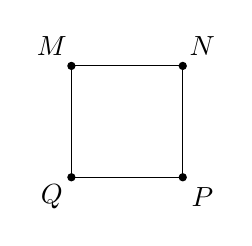
\begin{tikzpicture}[>=stealth,line join=round,line cap=round]
\foreach \diem/\i in {M/0,N/1,P/2,Q/3}{
\pgfmathsetmacro{\goc}{(360-360/4)*\i-(180-180/4)-90}
\fill(\goc:1)coordinate(\diem)circle(1.5pt)node[shift={(\goc:10pt)}]{$\diem$};
}
\draw[black] (M) \foreach \diem in {N,P,Q} {--(\diem)}--cycle;
\end{tikzpicture}
}
}
\end{ex}
\begin{ex}%[HK1, THPT Lê Quảng Chí, 2023]%[TVN-001, 10-11EX-HK1-2324]%[0H9V2-5]
trong mặt phẳng tọa độ $Oxy$, cho tam giác $ABC$ với $A(1;2)$, $B(-1;0)$, $C(3;2)$. Tìm tọa độ tâm đường tròn ngoại tiếp tam giác $ABC$.
\loigiai{
Gọi $I$ là tâm đường tròn ngoại tiếp tam giác $ABC$ và $I(x;y)$.\\
Từ giả thiết ta có \[\heva{&IA=IB\\&IA=IC}\Leftrightarrow \heva{&IA^2=IB^2\\&IA^2=IC^2.}\]
Ta có hệ phương trình sau
\[\heva{&(x-1)^2+(y-2)^2=(x+1)^2+(y-0)^2\\&(x-1)^2+(y-2)^2=(x-3)^2+(y-2)^2}\Leftrightarrow \heva{&-4x-4y=-4\\&4x+0y=8}\Leftrightarrow \heva{&x=2\\&y=-1.}\]
Tọa độ tâm $I(2;-1)$.
}
\end{ex}
\begin{ex}%[0D6V3-2]
Tại một lớp học chứng chỉ Tin học, nếu điểm trung bình $5$ bài kiểm tra của học viên lớn hơn hoặc bằng $85$ điểm thì học vìên sẽ được giảm $30\%$ học phí. An đã làm $4$ bài kiểm tra với kết quả (điểm số) lần lượt là $94$, $82$, $78$, $80$. Hỏi bài cuối cùng An cần đạt được ít nhất bao nhiêu điểm để được giảm $30\%$ học phí?
% \shortans{$91$}
\loigiai{
Giả sử bài kiểm tra cuối cùng An đạt được là $x\%$.\\
Khi đó trung bình $5$ bài kiểm tra của An là 
$$\overline{x}=\dfrac{94+82+78+80+x}{5}=\dfrac{x+334}{5}(\%)$$
Để được giảm học phí $30\%$ thì trung bình $5$ bài kiểm tra cần lớn hơn hoặc bằng $85\%$.\\
Khi đó ta có $\dfrac{x+334}{5}\ge 85\Leftrightarrow x\geq 91$.\\
Vậy bài cuối cùng An cần đạt được ít nhất $91\%$ để được giảm $30\%$ học phí.
}
\end{ex}
\Closesolutionfile{ans}
% \indapan{3}{ans/10-CK1-Chuyen-Hung-Vuong-Phan-3}